%\documentclass[preprint,tightenlines,showpacs,showkeys,floatfix,
%nofootinbib,superscriptaddress,fleqn]{revtex4} 
\documentclass[APS,floatfix,nofootinbib,superscriptaddress,fleqn,preprint]{revtex4} 
%\documentclass[aps,epsfig,tightlines,fleqn]{revtex4}
\usepackage[utf]{kotex}
\usepackage[HWP]{dhucs-interword}
\usepackage[dvips]{color}
\usepackage{graphicx}
\usepackage{bm}
%\usepackage{fancyhdr}
%\usepackage{dcolumn}
\usepackage{defcolor}
\usepackage{amsmath}
\usepackage{amsfonts}
\usepackage{amssymb}
\usepackage{amscd}
\usepackage{amsthm}
\usepackage[utf8]{inputenc}
 \usepackage{setspace}
%\pagestyle{fancy}

\begin{document}

\title{\Large 2021년 1학기 물리학 I: Quiz 2}
\author{김현철\footnote{Office: 5S-436D (면담시간 매주s
    화요일-16:00$\sim$20:00)}} 
\email{hchkim@inha.ac.kr}
\affiliation{Hadron Theory Group, Department of Physics, Inha University,
Incheon 402-751, Republic of Korea }
\date{Spring semester, 2022}


\vspace{1.cm}
\begin{abstract}
\noindent \textbf{ {\color{red}주의}: \color{blue} 단 한 번의 부정행위도 절대
  용납하지 않습니다. 적발 시, 학점은 F를 받게 됨은 물론이고,
  징계위원회에 회부합니다. One strike out임을 명심하세요.}\\
\\
문제는 다음 쪽부터 나옵니다.  \\ \\
{\bf Date:} 2021년 3월 7일 (월) 15:30-16:15 
\\
{\bf 학번:} \hspace{4cm}
{\bf 이름:} 

\end{abstract}
\maketitle

\noindent {\bf 문제 1 [20pt]}
그림~\ref{fig:1}과 같이 크기가 각각 1, 2, 4인 세 벡터 $\vec{A}$,
$\vec{B}$, $\vec{C}$가 같은 평면상에 놓여 있다. 벡터 $\vec{A}$와 벡터
$\vec{B}$는 서로 수직이고, 벡터 $\vec{B}$와 벡터 $\vec{C}$의 끼인각이 30°일 때,
벡터 $\vec{C}$는 벡터 $\vec{A}$와 벡터 $\vec{B}$를 사용하여
\begin{align*}
\vec{C} = \alpha \vec{A} + \beta\vec{B}  
\end{align*}
로 나타낼 수 있다. 두 상수 $\alpha$와 $\beta$를 구하여라. 
\begin{figure}[ht]
  \centering
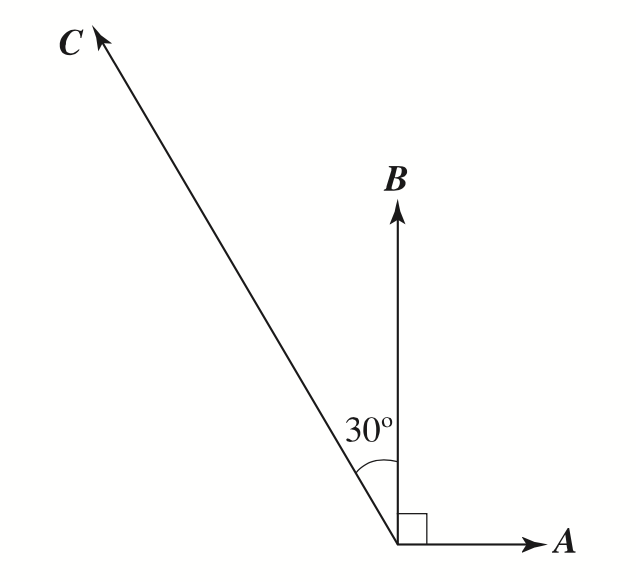
\includegraphics[scale=0.6]{Qfig3-1-20220307.png}  
  \caption{문제 1}
  \label{fig:1}
\end{figure} 

\noindent {\bf 해답} $\vec{A}$ 와 $\vec{B}$ 가 서로 수직이므로, $\vec{A} \cdot \vec{B} =0 $ 이다. 이는 다음을 의미한다.
\begin{align*}
  \vec{C} \cdot \vec{A} =\alpha\, \quad
  \vec{C} \cdot \vec{B} =\beta 
\end{align*}
스칼라곱의 정의를 이용하면 $\alpha$ 와 $\beta$ 를 구할 수 있다. 스칼라곱의 정의는 다음과 같다.
\begin{align*}
  \vec{A} \cdot \vec{B} = |\vec{A}||\vec{B}|\cos{\theta}
\end{align*}
이로부터 $\alpha$ 와 $\beta$ 는 다음과 같이 표현이 가능하다.
\begin{align*}
  \alpha &= |\vec{C}||\vec{A}|\cos{120^{\circ}} = 4 \times \left(-\frac{1}{2}\right) = -2 \\
  \beta &= |\vec{C}||\vec{B}|\cos{30^{\circ}} = 4 \times \frac{\sqrt{3}}{2} = 2\sqrt{3}
\end{align*}
따라서, $\vec{C}$ 는 다음과 같다.
\begin{align*}
  \vec{C} = -2 \vec{A} + 2\sqrt{3} \vec{B}
\end{align*}
\newpage

{\color{gray} [문제 풀이 쪽]}

\newpage 

\noindent {\bf 문제 2 [10pt]}
물리학자이자 의사였던 미공군 존 스탭(John P. Stapp) 대령은 제트기에서
조정사가 비상탈출을 했을 때 살아남을 수 있는지 직접 실험을
했다. 1954년 3월 19일, 그는 로켓을 단 차를 선로 위를 달릴 수 있도록
제작한 뒤,  1\,011 km/h의 속력으로 달렸다. 그리고 도착점에 거의 다
도달했을 때, 제동을 걸어 1.40 s만에 멈췄다. 
\begin{figure}[ht]
  \centering
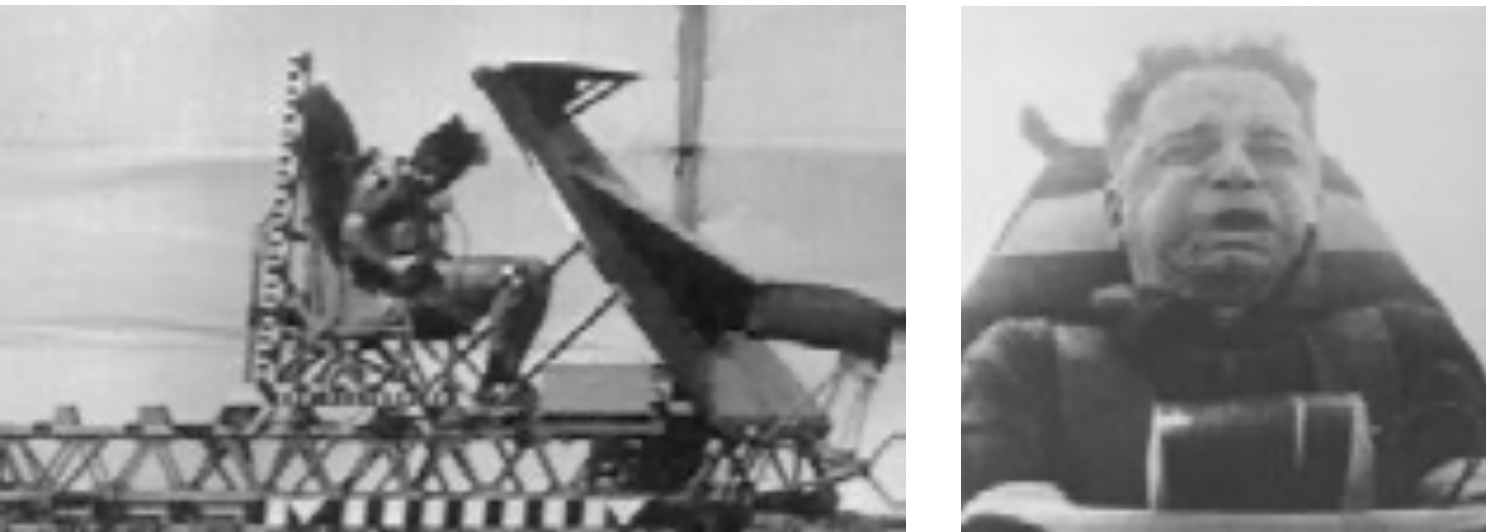
\includegraphics[scale=0.5]{Qfig3-2-20220307.png}  
  \caption{문제 2}
  \label{fig:2}
\end{figure}
\begin{itemize}
\item[(가)] 스탭 대령이 경험한 음의 가속도(감속도)를 구하여라. 구한
  가속도의 크기를 중력가속도 $g=9.80\,\mathrm{m/s^2}$로 나타내어라.
\item[(나)] 이 가속도를 받는 1.4 s  동안 스탭 대령이 간 거리는 얼마인가?
\end{itemize}
(이 실험으로 스탭 대령은 무릎뼈가 골절되고, 눈에 심각한 부상을 입어서
훗날 백내장으로 고생했다고 한다. 이 실험으로 스탭 대령은 자동차에 안전벨트를
도입하는 데 지대한 공을 세웠다.)
\newpage

{\color{gray} [문제 풀이 쪽]}

\newpage 

\noindent {\bf 문제 3 [10pt]} 
어떤 전투기가 그림~\ref{fig:2}에서처럼
35 m의 높이에서 $1\,300$ km/h의 속력으로 수평하게 날고 있다. $t=0$에서
이 전투기는 $\theta=4.3^\circ$의 각도로 기울어져 있는 언덕 위를
비행하기 시작했다. 만일 조종사가 이 전투기의 방향을 바꾸지 않는다면,
이 전투기는 언제 언덕과 충돌하게 되겠는가? 
\begin{figure}[ht]
  \centering
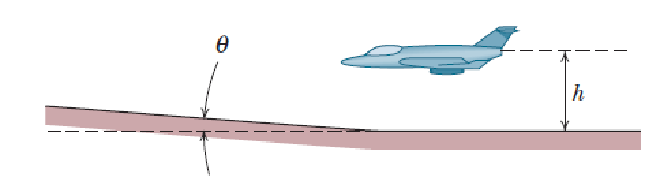
\includegraphics[scale=1.0]{Qfig3-2.pdf}  
  \caption{문제 1}
  \label{fig:1}
\end{figure} 

\newpage

{\color{gray} [문제 풀이 쪽]}

\newpage

\noindent {\bf 문제 4 [20pt]}
공사 중인 다리에서 볼트가 다리 아래 계곡으로 90 m 떨어진다.
\begin{itemize}
\item[(가)] 낙하거리의 마지막 20\% 지나는 데 걸리는 시간을 구하여라.
\item[(나)] 볼트가 낙하거리의 마지막 20\%를 들어설 때의 속력을
  구하여라.
\item[(다)] 다리 아래 계곡에 도달할 때 볼트의 속력을 구하여라.   
\end{itemize}


\newpage

{\color{gray} [문제 풀이 쪽]}

\newpage

\end{document}
